\documentclass[14pt,a4paper,report]{article}
\usepackage[a4paper, mag=1000, left=2.5cm, right=1cm, top=2cm, bottom=2cm, headsep=0.7cm, footskip=1cm]{geometry}
\usepackage[utf8]{inputenc}
\usepackage[english,russian]{babel}
\usepackage{indentfirst}
\usepackage[dvipsnames]{xcolor}
\usepackage[colorlinks]{hyperref}
\usepackage{listings} 
\usepackage{fancyhdr}
\usepackage{caption}
\usepackage{graphicx}
\usepackage{csquotes}
\usepackage{array}
\newcolumntype{P}[1]{>{\centering\arraybackslash}p{#1}}
\hypersetup{
	colorlinks = true,
	linkcolor  = black
}

\usepackage{titlesec}
\titleformat{\chapter}
{\Large\bfseries} % format
{}                % label
{0pt}             % sep
{\huge}           % before-code

\usepackage{accsupp}
\DeclareRobustCommand\squelch[1]{%
	\BeginAccSupp{method=plain,ActualText={}}#1\EndAccSupp{}}

\DeclareCaptionFont{white}{\color{white}} 

\usepackage{multido}
% to provide your syntax
\newcommand{\cmd}{-x-}
\newcommand{\Repeat}{\multido{\i=1+1}}


% Listing description
\usepackage{listings} 
\DeclareCaptionFormat{listing}{\colorbox{gray}{\parbox{\textwidth}{#1#2#3}}}
\captionsetup[lstlisting]{format=listing,labelfont=white,textfont=white}
\lstset{ 
	% Listing settings
	inputencoding = utf8,			
	extendedchars = \true, 
	keepspaces = true, 			  	 % Поддержка кириллицы и пробелов в комментариях
	language = C,            	 	 % Язык программирования (для подсветки)
	basicstyle = \small\sffamily, 	 % Размер и начертание шрифта для подсветки кода
	numbers = left,               	 % Где поставить нумерацию строк (слева\справа)
	numberstyle = \tiny,          	 % Размер шрифта для номеров строк
	stepnumber = 1,               	 % Размер шага между двумя номерами строк
	numbersep = 5pt,              	 % Как далеко отстоят номера строк от подсвечиваемого кода
	backgroundcolor = \color{white}, % Цвет фона подсветки - используем \usepackage{color}
	showspaces = false,           	 % Показывать или нет пробелы специальными отступами
	showstringspaces = false,    	 % Показывать или нет пробелы в строках
	showtabs = false,           	 % Показывать или нет табуляцию в строках
	frame = single,              	 % Рисовать рамку вокруг кода
	tabsize = 2,                  	 % Размер табуляции по умолчанию равен 2 пробелам
	captionpos = t,             	 % Позиция заголовка вверху [t] или внизу [b] 
	breaklines = true,           	 % Автоматически переносить строки (да\нет)
	breakatwhitespace = false,   	 % Переносить строки только если есть пробел
	escapeinside = {\%*}{*)}      	 % Если нужно добавить комментарии в коде
}

\begin{document}

\def\contentsname{Содержание}

% Titlepage
\begin{titlepage}
	\begin{center}
		\textsc{Санкт-Петербургский Политехнический 
			Университет Петра Великого\\[5mm]
			Кафедра компьютерных систем и программных технологий}
		
		\vfill
		
		\textbf{Аналитический отчет\\[3mm]
			Курс: «Интеллектуальные системы»\\[6mm]
			Тема: «Теория адаптивного резонанса»\\[35mm]
		}
	\end{center}
	
	\hfill
	\begin{minipage}{.4\textwidth}
		Выполнил студент:\\[2mm] 
		Бояркин Никита Сергеевич\\
		Группа: 13541/3\\[5mm]
		
		Проверил:\\[2mm] 
		Сазанов А.М.
	\end{minipage}
	\vfill
	\begin{center}
		Санкт-Петербург\\ \the\year\ г.
	\end{center}
\end{titlepage}

% Contents
\tableofcontents
\clearpage


\section{Введение}

Проблема \textit{стабильности-пластичности} является одной из самых сложных и трудно решаемых задач при построении искусственных систем, моделирующих восприятие. Характер восприятия внешнего мира живыми организмами (и, прежде всего, человеком) постоянно связан с решением дилеммы, является ли некоторый образ \textquote{новой} информацией, и следовательно реакция на него должна быть поисково-познавательной, с сохранением этого образа в памяти, либо этот образ является вариантом \textquote{старой}, уже знакомой картиной, и в этом случае реакция организма должна соответствовать ранее накопленному опыту \cite{cite-lek-narod} Таким образом, результирующее восприятие должно быть одновременно \textit{пластичным} (адаптированным к новой информации), и при этом \textit{стабильным} (не разрушающим память о старых образах).

Традиционные искусственные нейронные сети оказались не в состоянии решить проблему стабильности-пластичности \cite{cite-kgeu-adapt} Очень часто обучение новому образу уничтожает или изменяет результаты предшествующего
обучения.  Так, например, многослойный \textit{персептрон}, обучающийся по методу обратного распространения, запоминает весь пакет обучающей информации, при этом образы обучающей выборки предъявляются в процессе обучения многократно. Попытки затем обучить персептронновому образу приведут к модификации синаптических связей с неконтролируемым разрушением структуры памяти о предыдущих образах. 

Аналогичная ситуация имеет место и в сетях Кохонена и Хемминга, обучающихся на основе самоорганизации \cite{cite-kgeu-adapt} Данные сети всегда выдают положительный результат при классификации. Тем самым, эти нейронные сети не в состоянии отделить новые образы от искаженных или зашумленных версий старых образов. 

Исследования по проблеме стабильности-пластичности, выполненные в Центре Адаптивных Систем Бостонского университета под руководством Стефана Гроссберга, привели к построению теории адаптивного резонанса и созданию нейросетевых архитектур нового типа на ее основе \cite{cite-lek-narod}

Основная задача данного аналитического отчета -- анализ различных типов нейросетевых архитектур, в основе которых используется принцип адаптивного резонанса.

\section{Принцип адаптивного резонанса}

В основе \textit{принципа адаптивного резонанса} лежит использование нового принципа самоорганизации, который заключается в использовании слоя распознавания \textquote{снизу вверх} и слоя генерации \textquote{сверху вниз} \cite[с.~81]{book-simon-neural} Если входной и изученный образы совпадают, возникает состояние, называемое \textit{адаптивным резонансом} (усиление и продление нейронной активности).

Принцип работы нейросетевых архитектур на основе теории адаптивного резонанса заключается в том, что они имеют внутренний детектор новизны, сравнивающий предъявленный образ с содержимым памяти. При удачном поиске в памяти предъявленный образ классифицируется с одновременной уточняющей модификацией синаптических весов нейрона, выполнившего классификацию. О такой ситуации говорят, как о возникновении \textit{адаптивного резонанса} в сети в ответ на предъявление образа. Если резонанс не возникает в пределах некоторого заданного порогового уровня, то успешным считается тест новизны, и образ воспринимается сетью, как новый. Модификация весов нейронов, не испытавших резонанса, при этом не производится.

Важным понятием в теории адаптивного резонанса является так называемый \textit{шаблон критических черт} информации \cite{cite-lek-narod} Этот термин показывает, что не все черты (детали), представленные в некотором образе, являются существенными для системы восприятия. Результат распознавания определяется присутствием специфичных критических особенностей в образе. Рассмотрим это на примере.

\begin{figure}[h!]
	\centering
	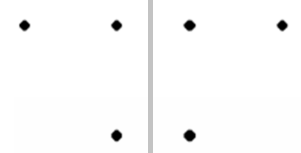
\includegraphics[scale = 0.80]{images/1.png}
	\caption{}
	\label{critical1}
\end{figure}

\clearpage

\begin{figure}[h!]
	\centering
	
\includegraphics[scale = 0.80]{images/2.png}
	\caption{}
	\label{critical2}
\end{figure}

В первом случае (Рис. \ref{critical1}) изменение в одной точке для правого и левого образа является критическим, поэтому правая и левая картинки считаются различными образами.

Во втором случае (Рис. \ref{critical2}) изменение в одной точке для правого и левого является не более чем шумом, и оба образа есть искаженные версии одного и того же изображения.

Следовательно, одна и та же черта образа может быть не существенной в одном случае, и критической в другом \cite{cite-kgeu-adapt} Задачей нейронной сети будет формирование правильной реакции в обоих случаях: \textquote{пластичное} решение о появлении нового образа для пары (Рис. \ref{critical1}) и \textquote{стабильное} решение о совпадении картинок (Рис. \ref{critical2}). При этом выделение критической части информации должно получаться автоматически в процессе работы и обучения сети, на основе ее индивидуального опыта.

В общем случае одного лишь перечисления черт может оказаться недостаточно для успешного функционирования искусственной нейронной системы, критическими могут оказаться специфические связи между несколькими отдельными чертами.

\section{Архитектура ART}

Разработано несколько видов нейросетей на основе адаптивной резонансной теории, в частности, сети ART-1 и ART-2. ART-1 предназначена для работы с двоичными входными изображениями или векторами, а ART-2 - для классификации как двоичных, так и непрерывнозначных векторов \cite{cite-life-prog} 

\subsection{Базовая архитектура ART}

Хотя детали архитектуры и алгоритмов работы для ART-1 и ART-2 различны, однако они имеют общую базовую архитектуру (Рис. \ref{art-base}).

\begin{figure}[h!]
	\centering
	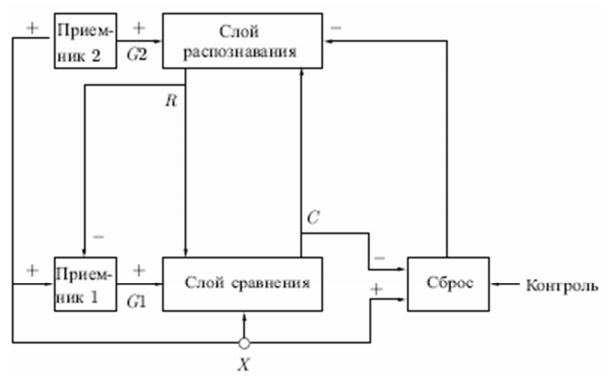
\includegraphics[scale = 0.80]{images/3.png}
	\caption{Базовая архитектура ART}
	\label{art-base}
\end{figure}

Базовая архитектура ART (Рис. \ref{art-base}) включает два слоя нейронов: слой сравнения и слой распознавания. Приемники обеспечивают управляющую функциональность, необходимую для обучения и классификации.

\subsubsection{Слой сравнения}

\textit{Слой сравнения} получает двоичный входной вектор X и первоначально пропускает его неизмененным для формирования выходного вектора C. На более поздней фазе в распознающем слое вырабатывается двоичный вектор R, модифицирующий вектор C \cite{cite-kgeu-adapt}

Каждый нейрон в слое сравнения (Рис. \ref{art-compare}) получает три двоичных входа:

\begin{itemize}
	\item Компонента Xi входного вектора X.
	\item Сигнал обратной связи Ri -- взвешенная сумма выходов распознающего слоя
	\item Вход от приемника.
\end{itemize}

\begin{figure}[h!]
	\centering
	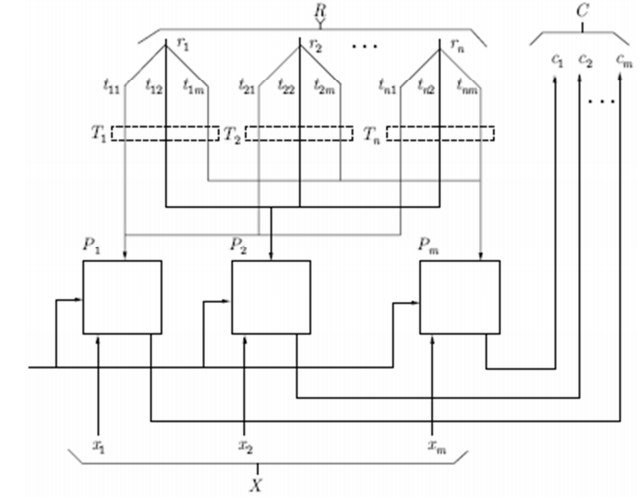
\includegraphics[scale = 0.90]{images/4.png}
	\caption{Слой сравнения}
	\label{art-compare}
\end{figure}

Чтобы получить на выходе нейрона единичное значение, как минимум два из трех его входов должны равняться единице; в противном случае его выход будет нулевым. Таким образом, реализуется правило двух третей. Первоначально выходной сигнал G1 приемника 1 установлен в единицу, обеспечивая один из входов, необходимых для возбуждения нейронов, а все компоненты вектора R установлены в 0; следовательно, в этот момент вектор C идентичен двоичному входному вектору X. 

\subsubsection{Слой распознавания}

\textit{Слой распознавания} осуществляет классификацию входных векторов. Каждый нейрон в слое распознавания имеет соответствующий вектор весов Bj. Только один нейрон с весовым вектором, наиболее соответствующим входному вектору, возбуждается; все остальные заторможены. 

Как показано на (Рис. \ref{art-recognition}), нейрон в распознающем слое имеет максимальную реакцию, если вектор C, являющийся выходом слоя сравнения, соответствует набору его весов; следовательно, веса представляют запомненный образ или экземпляр для категории входных векторов. Такие веса являются действительными числами, а не двоичными величинами. Двоичная версия этого образа также запоминается в соответствующем наборе весов слоя сравнения (Рис. \ref{art-compare}); этот набор состоит из весов связей, соединяющих определенные нейроны слоя распознавания, по одному весу на каждый нейрон слоя сравнения.

\begin{figure}[h!]
	\centering
	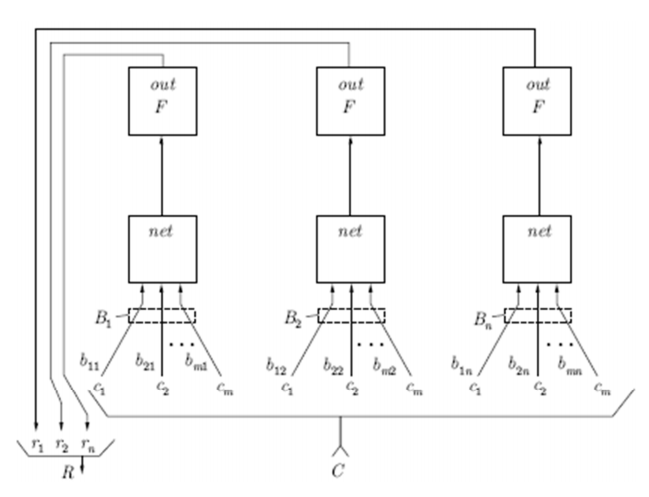
\includegraphics[scale = 0.88]{images/5.png}
	\caption{Слой распознавания}
	\label{art-recognition}
\end{figure}

В процессе функционирования каждый нейрон слоя распознавания вычисляет свертку вектора собственных весов и входного вектора C. Нейрон, веса которого наиболее близки вектору C, будет иметь самый большой выход, тем самым выигрывая соревнование и одновременно затормаживая все остальные нейроны в слое. Нейроны внутри слоя распознавания взаимно соединены в латерально-тормозящую сеть. В простейшем случае предусматривается, что только один нейрон в слое возбуждается в каждый момент времени (только нейрон с наивысшим уровнем активации будет иметь единичный выход, все остальные нейроны будут иметь нулевой выход).

\subsubsection{Управляющие модули}

Выход G2 \textit{приемника 2} равен единице, если входной вектор X имеет хотя бы одну единичную компоненту (G2 является логическим или от вектора X).

Выход G1 \textit{приемника 1} равен единице, если входной вектор X имеет хотя бы одну единичную компоненту, однако, если хотя бы одна компонента вектора R равна единице, G1 устанавливается в нуль. Таблица, определяющая эти соотношения: 

\begin{table}[h!]
	\centering
	\bgroup
	\def\arraystretch{1}
	\begin{tabular}{ | P{3.8cm} | P{3.8cm} | P{1.8cm} | }
		\hline
		ИЛИ от компонента вектора X & ИЛИ от компонента вектора R & \textbf{G1} 
		\\ \hline
		
		0 & 0 & \textbf{0} \\ \hline
		
		1 & 0 & \textbf{1} \\ \hline
		
		1 & 1 & \textbf{0} \\ \hline
		
		1 & 1 & \textbf{0} \\ \hline
		
	\end{tabular}
	\egroup
	\caption{Таблица соотношений приемника 1}
	\label{table:1}
\end{table}

В процессе функционирования \textit{модуль сброса} вычисляет сходство как отношение количества единиц в векторе X к их количеству в векторе C. Если это отношение ниже значения параметра сходства, вырабатывается сигнал сброса. 


\subsection{Классификация в сетях ART}

Рассмотрим подробнее процесс классификации в сетях ART. 

\subsubsection{Фаза инициализации}

Нулевые значения компонент входного вектора X устанавливают сигнал нейрона приемника 2 в нуль, одновременно устанавливая в нуль выходы нейронов слоя распознавания. При возникновении ненулевых значений X, оба сигнала управления (G1 и G2) устанавливаются равными единице. При этом по правилу двух третей выходы нейронов слоя сравнения C в точности равны компонентам X.

Вектор C поступает на входы нейронов слоя распознавания, которые в конкурентной борьбе определяют нейрон-победитель, описывающий предполагаемый результат классификации. В итоге выходной вектор R слоя распознавания содержит ровно одну единичную компоненту, остальные значения равны нулю. Ненулевой выход нейрона-победителя устанавливает в нуль сигнал управления 1: G1=0. По обратной связи нейрон-победитель посылает сигналы в слой сравнения, и начинается \textit{фаза сравнения} \cite{cite-lek-narod}

Параметр сходства $\rho$ устанавливается в диапазоне от 0 до 1 в зависимости от требуемой степени сходства
между запомненным образом и входным вектором. При высоких значениях сеть относит к одному классу
только очень слабо отличающиеся образы. С другой стороны, малое значение $\rho$ заставляет сеть группировать образы, которые имеют слабое сходство между собой. Для выработки точной классификации полезна возможность изменять коэффициент сходства на протяжении процесса обучения, обеспечивая только грубую классификацию в начале процесса обучения и затем постепенно увеличивая коэффициент сходства. 

\subsubsection{Фаза распознавания}

Появление на входе сети входного вектора X инициализирует \textit{фазу распознавания}. Так как вначале выходной вектор слоя распознавания отсутствует, сигнал G1 устанавливается в 1 функцией ИЛИ вектора X, обеспечивая все нейроны слоя сравнения одним из двух входов, необходимых для их возбуждения (как требует правило двух третей). В результате любая компонента вектора X, равная единице, обеспечивает второй единичный вход, заставляя соответствующий нейрон слоя сравнения возбуждаться и устанавливая его выход в единицу. Таким образом, в этот момент времени вектор C идентичен вектору X. 

Распознавание реализуется вычислением свертки для каждого нейрона слоя распознавания, определяемой следующим выражением:

\begin{figure}[h!]
	\centering
	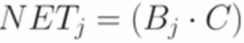
\includegraphics[scale = 0.55]{images/f_4.png}
\end{figure}

Где -- Bj весовой вектор, соответствующий нейрону j в слое распознавания, C -- выходной вектор нейронов слоя сравнения (в этот C момент равно X), NETj — возбуждение нейрона j в слое распознавания. 
нейрона в слое распознавания.

F является пороговой функцией, определяемой следующим образом:

\begin{figure}[h!]
	\centering
	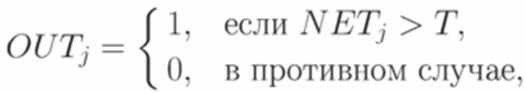
\includegraphics[scale = 0.55]{images/f_5.png}
\end{figure}

Где T -- пороговое значение.

Принято, что латеральное торможение существует, но игнорируется здесь для сохранения простоты выражения \cite{cite-kgeu-adapt} Торможение является причиной того, что только нейрон с максимальным значением NET будет иметь выход, равный единице; все остальные нейроны будут иметь нулевой выход. Можно рассмотреть системы, в которых в распознающем слое возбуждаются несколько нейронов в каждый момент времени, однако это выходит за рамки данной работы.

\subsubsection{Фаза сравнения}

В слое сравнения веер сигналов отклика слоя распознавания сравнивается с компонентами вектора X. Выход слоя сравнения C теперь содержит единичные компоненты только в тех позициях, в которых единицы имеются и у входного вектора X и у вектора обратной связи P. Если в результате сравнения векторов C и X не будет обнаружено значительных отличий, то нейрон сброса остается неактивным. Вектор C вновь вызовет возбуждение того-же нейрона-победителя в слое распознавания, что и удачно завершит процесс классификации. В противном случае будет выработан сигнал сброса, который затормозит нейрон-победитель в слое распознавания, и начнется \textit{фаза поиска} \cite{cite-lek-narod}

На этой фазе сигнал обратной связи от слоя распознавания устанавливает в нуль; правило двух третей позволяет возбуждаться только тем нейронам, которые имеют соответствующие компоненты векторов P и X, равные единице. 

Блок сброса сравнивает вектор C и входной вектор X, вырабатывая сигнал сброса, когда их сходство S ниже порога сходства. Вычисление этого сходства упрощается тем, что оба вектора являются двоичными (все элементы либо 0, либо 1). Следующая процедура проводит требуемое вычисление сходства:

\begin{itemize}
	\item Вычислить D -- количество единиц в векторе X.
	\item Вычислить N -- количество единиц в векторе C.
	\item Вычислить сходство $S=N/D$
\end{itemize}

Например, примем, что

$X=\{1, 0, 1, 1, 1, 0, 1\} \rightarrow D = 5$

$C=\{0, 0, 1, 1, 1, 0, 1\} \rightarrow N = 4$

$S=N/D=4/5=0.8$

Может изменяться от 1 (наилучшее соответствие) до 0 (наихудшее соответствие).

Заметим, что правило двух третей делает С логическим произведением входного вектора Х и вектора Р \cite{cite-techn-adapt} Однако Р равен Тj, весовому вектору выигравшего соревнование нейрона. Таким образом, D может быть определено как количество единиц в логическом произведении векторов Тj и X.

\subsubsection{Фаза поиска}

В результате действия тормозящего сигнала сброса все нейроны слоя распознавания получат нулевые выходы, и, следовательно, нейрон приемника 1 примет единичное значение активности. Снова выходной сигнал слоя сравнения C установится равным в точности X, как и в начале работы сети. Однако теперь в конкурентной борьбе в слое распознавания предыдущий нейрон-победитель не участвует, и будет найдена новая категория - кандидат. После чего опять повторяется фаза сравнения.

Итерационный процесс поиска завершается двумя возможными способами:

\begin{itemize}
	\item Найдется запомненная категория, сходство которой с входным вектором X будет достаточным для успешной классификации. После этого происходит обучающий цикл, в котором модифицируются веса bi и ti векторов B и T возбужденного нейрона, осуществившего классификацию.
	\item В процессе поиска все запомненные категории окажутся проверенными, но ни одна из них не дала требуемого сходства. В этом случае входной образ X об'является новым для нейросети, и ему выделяется новый нейрон в слое распознавания. Весовые вектора этого нейрона B и T устанавливаются равными вектору X.
\end{itemize}

Отметим, что после относительной стабилизации процесса обучения классификация выполняется без фазы поиска. В этом случае говорят, что формируется прямой доступ к памяти. Возникновение в процессе обучения прямого доступа доказывается в теории АРТ \cite{cite-lek-narod}

Если сходство S выигравшего нейрона превышает параметр сходства, поиск не требуется. Однако если сеть предварительно была обучена, появление на входе вектора, не идентичного ни одному из предъявленных ранее, может возбудить в слое распознавания нейрон со сходством ниже требуемого уровня. В соответствии с алгоритмом обучения возможно, что другой нейрон в слое распознавания будет обеспечивать более хорошее соответствие, превышая требуемый уровень сходства несмотря на то, что свертка между его весовым вектором и входным вектором может иметь меньшее значение. Пример такой ситуации показан ниже.
 
Если сходство ниже требуемого уровня, запомненные образы могут быть просмотрены с целью поиска, наиболее соответствующего входному вектору образа. Если такой образ отсутствует, вводится новый несвязанный нейрон, который в дальнейшем будет обучен. Для инициализации поиска сигнал сброса тормозит возбужденный нейрон в слое распознавания на время проведения поиска, сигнал G1 устанавливается в единицу и другой нейрон в слое распознавания выигрывает соревнование. Его запомненный образ затем проверяется на сходство и процесс повторяется до тех пор, пока конкуренцию не выиграет нейрон из слоя распознавания со сходством, большим требуемого уровня (успешный поиск), либо пока все связанные нейроны не будут проверены и заторможены (неудачный поиск).
 
Неудачный поиск будет автоматически завершаться на несвязанном нейроне, так как его веса все равны единице, своему начальному значению. Поэтому правило двух третей приведет к идентичности вектора С входному вектору X, сходство S примет значение единицы и критерий сходства будет удовлетворен.

\subsection{Обучение сети ART}

Обучение представляет собой процесс, в котором набор входных векторов подается последовательно на вход сети, а веса сети изменяются при этом таким образом, чтобы сходные векторы активизировали соответствующие им нейроны. Заметим, что это - неуправляемое обучение, здесь нет учителя и нет целевого вектора, определяющего требуемый ответ.

Различают два вида обучения: медленное и быстрое. При медленном обучении входной вектор предъявляется настолько кратковременно, что веса сети не успевают достигнуть своих ассимптотических значений при единичном предъявлении. В этом случае значения весов будут определяться, скорее, статистическими характеристиками входных векторов, чем характеристиками какого-то одного входного вектора. Динамика сети в процессе медленного обучения описывается дифференциальными уравнениями \cite{cite-kgeu-adapt}

Быстрое обучение является специальным случаем медленного обучения, когда входной вектор прикладывается на достаточно длительный срок, чтобы позволить весам приблизиться к их окончательным значениям. В этом случае процесс обучения описывается только алгебраическими выражениями. Кроме того, компоненты весовых векторов принимают двоичные значения, в отличие от непрерывного диапазона значений, требуемого в случае быстрого обучения. В данной лекции мы опишем только быстрое обучение. 

В общих чертах сеть обучается посредством изменения весов таким образом, что предъявление сети входного вектора заставляет сеть активизировать нейроны в слое распознавания, связанные с сходным запомненным вектором \cite{cite-techn-adapt} Кроме этого, обучение проводится в форме, не разрушающей запомненные ранее образы, предотвращая тем самым временную нестабильность. Эта задача управляется на уровне выбора критерия сходства. Новый входной образ (который сеть не видела раньше) не будет соответствовать запомненным образам с точки зрения параметра сходства, тем самым формируя новый запоминаемый образ. Входной образ, в достаточной степени соответствующий одному из запомненных образов, не будет формировать нового экземпляра, он просто будет модифицировать тот, на который он похож. Таким образом при соответствующем выборе критерия сходства предотвращается запоминание ранее изученных образов и временная нестабильность.

\begin{figure}[h!]
	\centering
	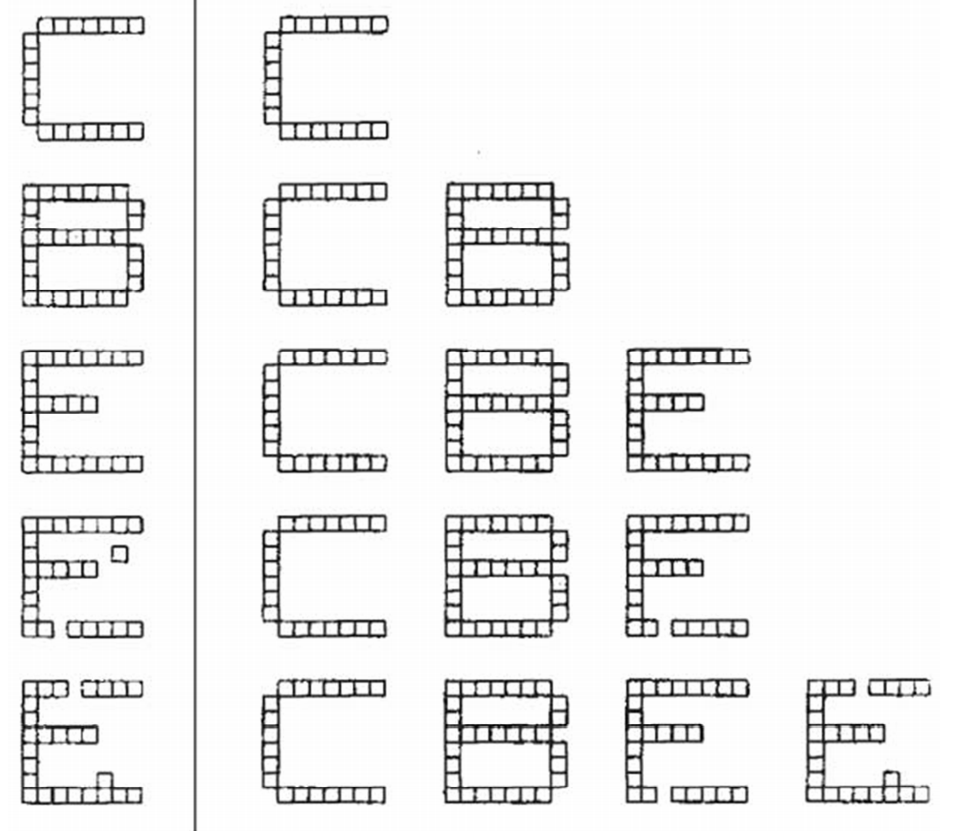
\includegraphics[scale = 0.60]{images/6.png}
	\caption{Процесс обучения ART}
	\label{art-study}
\end{figure}

На рис. \ref{art-study} показан типичный сеанс обучения сети APT. Буквы показаны состоящими из маленьких квадратов, каждая буква размерностью 8x8. Каждый квадрат в левой части представляет компоненту вектора Х с единичным значением, не показанные квадраты являются компонентами с нулевыми значениями. Буквы справа представляют запомненные образы, каждый является набором величин компонент вектора Тj.

Вначале на вход заново проинициированной системы подается буква \textquote{С}. Так как отсутствуют запомненные образы, фаза поиска заканчивается неуспешно; новый нейрон выделяется в слое распознавания, и веса Тj устанавливаются равными соответствующим компонентам входного вектора, при этом веса Вj представляют масштабированную версию входного вектора.

Далее предъявляется буква \textquote{В}. Она также вызывает неуспешное окончание фазы поиска и распределение нового нейрона. Аналогичный процесс повторяется для буквы \textquote{Е}. Затем слабо искаженная версия буквы «Е» подается на вход сети. Она достаточно точно соответствует запомненной букве \textquote{Е}, чтобы выдержать проверку на сходство, поэтому используется для обучения сети. Отсутствующий пиксель в нижней ножке буквы \textquote{Е} устанавливает в 0 соответствующую компоненту вектора С, заставляя обучающий алгоритм установить этот вес запомненного образа в нуль, тем самым воспроизводя искажения в запомненном образе. Дополнительный изолированный квадрат не изменяет запомненного образа, так как не соответствует единице в запомненном образе.

Четвертым символом является буква \textquote{Е} с двумя различными искажениями. Она не соответствует ранее запомненному образу (S меньше чем $\rho$), поэтому для ее запоминания выделяется новый нейрон.

Этот пример иллюстрирует важность выбора корректного значения критерия сходства. Если значение критерия слишком велико, большинство образов не будут подтверждать сходство с ранее запомненными и сеть будет выделять новый нейрон для каждого из них. Это приводит к плохому обобщению в сети, в результате даже незначительные изменения одного образа будут создавать отдельные новые категории. Количество категорий увеличивается, все доступные нейроны распределяются, и способность системы к восприятию новых данных теряется \cite{cite-techn-adapt} Наоборот, если критерий сходства слишком мал, сильно различающиеся образы будут группироваться вместе, искажая запомненный образ до тех пор, пока в результате не получится очень малое сходство с одним из них.

\subsection{Характеристики ART}

Системы APT имеют ряд важных характеристик, не являющихся очевидными. Формулы и алгоритмы могут казаться произвольными, в то время как в действительности они были тщательно отобраны с целью удовлетворения требований теорем относительно производительности систем APT. В данном разделе описываются некоторые алгоритмы APT, раскрывающие отдельные вопросы инициализации и обучения.

\subsubsection{Инициализация весовых векторов Т}

Из ранее рассмотренного примера обучения сети можно было видеть, что правило двух третей приводит к вычислению вектора С как функции И между входным вектором Х и выигравшим соревнование запомненным вектором Тj \cite{cite-techn-adapt} Следовательно, любая компонента вектора С будет равна единице в том случае, если соответствующие компоненты обоих векторов равны единице. После обучения эти компоненты вектора Тj остаются единичными; все остальные устанавливаются в нуль.

Это объясняет, почему веса tij должны инициализироваться единичными значениями. Если бы они были проинициализированы нулевыми значениями, все компоненты вектора С были бы нулевыми независимо от значений компонент входного вектора, и обучающий алгоритм предохранял бы веса от изменения их нулевых значений.

Обучение может рассматриваться как процесс \textquote{сокращения} компонент запомненных векторов, которые не соответствуют входным векторам \cite{cite-kgeu-adapt} Этот процесс необратим, если вес однажды установлен в нуль, обучающий алгоритм никогда не восстановит его единичное значение.

Это свойство имеет важное отношение к процессу обучения. Предположим, что группа точно соответствующих векторов должна быть классифицирована к одной категории, определяемой возбуждением одного нейрона в слое распознавания. Если эти вектора последовательно предъявляются сети, при предъявлении первого будет распределяться нейрон распознающего слоя, его веса будут обучены с целью соответствия входному вектору. Обучение при предъявлении остальных векторов будет приводить к обнулению весов в тех позициях, которые имеют нулевые значения в любом из входных векторов \cite{cite-techn-adapt} Таким образом, запомненный вектор представляет собой логическое пересечение всех обучающих векторов и может включать существенные характеристики данной категории весов. Новый вектор, включающий только существенные характеристики, будет соответствовать этой категории. Таким образом, сеть корректно распознает образ, никогда не виденный ранее, т. е. реализуется возможность, напоминающая процесс восприятия человека.

\subsubsection{Настройка весовых векторов Вj}

Выражение, описывающее процесс настройки весов является центральным для описания процесса функционирования сетей APT:

\begin{figure}[h!]
	\centering
	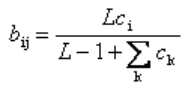
\includegraphics[scale = 0.90]{images/f_1.png}
\end{figure}

Сумма в знаменателе представляет собой количество единиц на выходе слоя сравнения. Эта величина может быть рассмотрена как \textquote{размер} этого вектора. В такой интерпретации «большие» векторы С производят более маленькие величины весов bij, чем \textquote{маленькие} вектора С. Это свойство самомасштабирования делает возможным разделение двух векторов в случае, когда один вектор является поднабором другого; т. е. когда набор единичных компонент одного вектора составляет подмножество единичных компонент другого.

Чтобы продемонстрировать проблему, возникающую при отсутствии масштабирования, используемого в вышеприведенном выражении, предположим, что сеть обучена двум приведенным ниже входным векторам, при этом каждому распределен нейрон в слое распознавания.

Заметим, что Х1 является поднабором Х2. В отсутствие свойства масштабирования веса bij и tij получат значения, идентичные значениям входных векторов. Если начальные значения выбраны равными 1 и 0, веса образов будут иметь следующие значения: если Х прикладывается повторно, оба нейрона в слое распознавания получают одинаковые активации; следовательно, нейрон 2, ошибочный нейрон, выиграет конкуренцию \cite{cite-techn-adapt}

Кроме выполнения некорректной классификации, может быть нарушен процесс обучения. Так как Т2 равно 1 1 1 0 0, только первая единица соответствует единице входного вектора, и С устанавливается в 1 0 0 0 0, критерий сходства удовлетворяется и алгоритм обучения устанавливает вторую и третью единицы векторов Т2 и В2 в нуль, разрушая запомненный образ.

Масштабирование весов bij предотвращает это нежелательное поведение. Предположим, что в вышеприведенном выражении используется значение L=2, тем самым определяя следующую формулу:

\begin{figure}[h!]
	\centering
	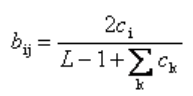
\includegraphics[scale = 0.90]{images/f_2.png}
\end{figure}

Подавая на вход сети вектор Х1 , получим возбуждающее воздействие 1,0 для нейрона 1 в слое распознавания и 1/2 для нейрона 2; таким образом, нейрон 1 (правильный) выиграет соревнование. Аналогично предъявление вектора Х2 вызовет уровень возбуждения 1,0 для нейрона 1 и 3/2 для нейрона 2, тем самым снова правильно выбирая победителя.

\subsubsection{Инициализация весов bij}

Инициализация весов bij малыми значениями является существенной для корректного функционирования систем APT. Если они слишком большие, входной вектора который ранее был запомнен, будет скорее активизировать несвязанный нейрон, чем ранее обученный. Следующее выражение выражение, определяет начальные значения весов:

\begin{figure}[h!]
	\centering
	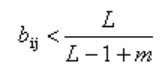
\includegraphics[scale = 0.97]{images/f_3.png}, для всех i, j
\end{figure}

Установка этих весов в малые величины гарантирует, что несвязанные нейроны не будут получать возбуждения большего, чем обученные нейроны в слое распознавания \cite{cite-techn-adapt} Используя предыдущий пример с L=2, m=5 и bij<1/3, произвольно установим bij=1/6. С такими весами предъявление вектора, которому сеть была ранее обучена, приведет к более высокому уровню активации для правильно обученного нейрона в слое распознавания, чем для несвязанного нейрона. Например, для несвязанного нейрона Х1 будет производить возбуждение 1/6, в то время как Х2 будет производить возбуждение 1/2; и то и другое ниже возбуждения для обученных нейронов.

\subsection{Проблема производительности}

Описанная сеть должна производить последовательный поиск среди всех запомненных образов. В аналоговых реализациях это будет происходить очень быстро; однако при моделировании на обычных цифровых компьютерах этот процесс может оказаться очень длительным. Если же сеть APT реализуется на параллельных процессорах, все свертки на распознающем уровне могут вычисляться одновременно. В этом случае поиск может быть очень быстрым.

Время, необходимое для стабилизации сети с латеральным торможением, может быть длительным при моделировании на последовательных цифровых компьютерах. Чтобы выбрать победителя в процессе латерального торможения, все нейроны в слое должны быть вовлечены в одновременные вычисления и передачу \cite{cite-scritub-adapt} Это может потребовать проведения большого объема вычислений перед достижением сходимости. Латеральные тормозящие сети, аналогичные используемым в неокогнитронах, могут существенно сократить это время.

\subsection{Типовые задачи ART}

Типовые задачи, решаемые в контексте ИНС и представляющие научный и практический интерес, можно подразделить следующим образом: 

\begin{itemize}
	\item \textit{Классификация образов}. Задача состоит в указании принадлежности входного образа (например, речевого сигнала или рукописного символа), представленного вектором признаков, одному или нескольким предварительно определенным классам. К известным приложениям относятся распознавание букв, распознавание речи, классификация сигнала электрокардиограммы, классификация клеток крови \cite{book-bikanov}
	
	\item \textit{Кластеризация/категоризация}. При решении задачи кластеризации, которая известна также как классификация образов «без учителя», отсутствует обучающая выборка с метками классов. Алгоритм кластеризации основан на подобии образов и размещает близкие образы в один кластер. Кластеризация применяется для извлечения знаний, сжатия данных и исследования их свойств \cite{book-bikanov}
\end{itemize}

\subsection{Архитектуры производных ART сетей}

Сети ART-1 получили заслуженное развитие. В данном разделе рассматриваются модифицированные версии архитектуры ART-1, для которых в большей степени справедливы базовые принципы описанные в предыдущих разделах.

Полная классификация производных ART сетей представлена на рис. \ref{art-tree}.

\begin{figure}[h!]
	\centering
	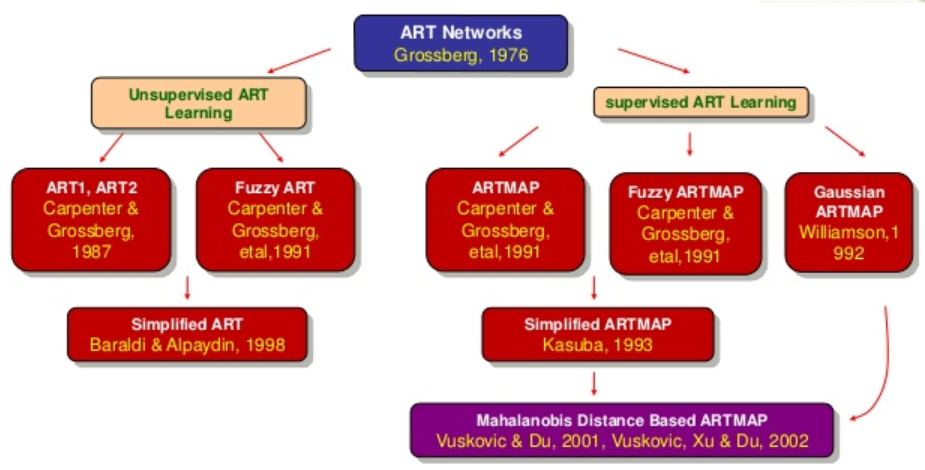
\includegraphics[scale = 0.72]{images/7.png}
	\caption{Классификация производных ART архитектур}
	\label{art-tree}
\end{figure}

\subsubsection{Архитектура ART-2}

Основной отличительной чертой нейронной сети ART-2 является возможность работы с аналоговыми векторами и сигналами. По сравнению с ART-1 в архитектуре сети сделаны некоторые изменения, позволяющие отдельным подсистемам функционировать асинхронно, что принципиально для аппаратных реализаций \cite{cite-lek-narod}

Важным отличием аналоговых сигналов от битовых является принципиальная возможность аналоговых векторов быть сколь угодно близкими друг к другу (в то время как простанство битовых векторов дискретно). Это накладывает дополнительные требования на функционирование нейронов слоя сравнения - требуется более тонкий и чувствительный механизм для выделения областей резонанса. Общим решением здесь является переход к многослойной архитектуре, с все более точной настройкой при переходе от слоя к слою, что и применено в ART-2. Функционирование слоя распознавания принципиально не изменяется.

\subsubsection{Архитектура ART-3}

Следующим шагом в развитии ART явилась сеть ART-3. Особенности обучения нейронов сетей ART-1 и ART-2 не позволяют использовать эти сети, как элементы более крупных иерархических нейросистем, в частности, компоновать из них многослойные сети. Это затрудняет представление в ART иерархически организованной информации, что характерно для систем восприятия человека и животных.

Эти проблемы решены в сети ART-3, которая выступает как многослойная архитектура \cite{cite-lek-narod} При переходе от слоя к слою происходит контрастирование входных образов и запоминание их в виде все более общих категорий. При этом основной задачей каждого отдельного слоя является сжатие входящей информации. Образ входит в адаптирующийся резонанс между некоторой парой слоев, в дальнейшем этот резонанс распространяется на следующие слои иерархии. В ART-1 и ART-2 недостаточный уровень резонанса приводил к генерации сигнала сброса, что приводило к полному торможению слоя распознавания. В случае многослойной сети ART-3 подобное недопустимо, так как при этом разрывается поток информации. Поэтому в ART-3 введен специальный механизм — зависимость активности синапсов обратных связей от времени -- аналогичный рефрактерному торможению биологического нейрона после передачи возбуждения \cite{cite-kgeu-adapt} Поэтому вместо полного сброса сигнала происходит торможение синаптических сигналов обратной связи, и слой сравнения получает исходное состояние возбуждения для выполнения фазы поиска нового резонанса. 

Интересным предложением является также использование в многослойной иерархии слоев, которые не являются слоями ART, а принадлежат некоторой другой архитектуре. В этом случае система получается гибридной, что может привести к возникновению новых полезных свойств.

\subsubsection{Архитектура ARTMAP}

Архитектура ARTMAP объединяют элементы обучения и самообучения (или обучения с поощрением и без поощрения, Supervised and Unsupervised Training). Для этого обычно формируется комбинация из двух ART-сетей \cite{cite-window-adapt}

\subsubsection{Архитектура FUZZY-ART}

FUZZY-ART представляет собой прямое расширение ART-1-сетей средствами нечеткой логики (Fuzzy Logic) \cite{cite-window-adapt} В них применяются следующие операторы:

\begin{itemize}
	\item для определения класса образов в слое распознавания;
	\item для расчета степени сходства (Reset-критерий);
	\item для адаптации весов;
\end{itemize}	

В результате данной модификации ART-1-сети могут быть использованы для обработки не бинарных, а действительных входных векторов.

\section{Заключение}

В ходе исследования были выявлены некоторые основополагающие характеристики теории адаптивного резонанса:

\begin{itemize}
	\item После стабилизации процесса обучения предъявление одного из обучающих векторов будет активизировать требуемый нейрон слоя распознавания без поиска. Эта характеристика \textquote{прямого доступа} определяет быстрый доступ к предварительно изученным образам.
	\item Процесс поиска является устойчивым. После определения выигравшего нейрона в сети не будет возбуждений других нейронов в результате изменения векторов выхода слоя сравнения С; только сигнал сброса может вызвать такие изменения.
	\item Процесс обучения является устойчивым. Обучение не будет вызывать переключения с одного возбужденного нейрона слоя распознавания на другой.
	\item Процесс обучения конечен. Любая последовательность произвольных входных векторов будет производить стабильный набор весов после конечного количества обучающих серий; повторяющиеся последовательности обучающих векторов не будут приводить к циклическому изменению весов.
\end{itemize}

Идея адаптивного резонанса позволила объяснить Гроссбергу некоторые особенности человеческого восприятия, например задержку в осознании сенсорной информации по сравнению со временем, требуемым для прохождения сигнала по зрительному или слуховому тракту. Эта задержка есть время, необходимое для установления резонанса и зависящее как от силы ожиданий, так и от степени неопределенности воспринимаемой информации.

С помощью адаптивного резонанса можно объяснить и тот факт, что на то, чтобы в первый раз увидеть объект, спрятанный на изображении-головоломке, уходит значительно больше времени, чем на его восприятие в последующие разы. На таких изображениях присутствует объект, складывающийся из каких-то других случайных объектов, но чтобы его увидеть, необходимы заметные усилия со стороны зрительной системы. Для распознавания спрятанного объекта требуется правильно сгруппировать видимые объекты, что требует большого перебора вариантов. Если бы обработка сенсорной информации шла строго снизу вверх, то зрительной системе пришлось бы каждый раз заново решать эту задачу. Второй раз взглянув на то же изображение, человек мог бы помнить, что на нем изображено, но не видеть этого до тех пор, пока нужная комбинация снова не нашлась. Однако распространение информации сверху вниз позволяет эффективно отсеивать неперспективные гипотезы нижних уровней, эффективно направляя поиск правильной интерпретации изображения.

Трудности в теории адаптивного резонанса возникают не только для верхних уровней восприятия. Не решается и проблема инвариантного распознавания. Речь здесь идет лишь о разрешении неопределенности для зашумленных образов, тогда как даже простое смещение объекта препятствует распознаванию.

Первоначальная простая архитектура нейронной сети в теории адаптивного резонанса впоследствии была сильно усложнена, и некоторые недостатки были устранены, однако принципиальные проблемы, связанные с отсутствием инвариантности и ограничением на число гипотез, решены не были \cite{cite-aideus-adapt}

Итак, первичная обработка зрительной информации, распознавание зрительных образов, обработка потоков звуковой информации, распознавание речи, управление движением глаз и представление информации в соматосенсорной коре, все эти задачи могут решаться различными типами сетей ART. Из этих результатов следует, что какая-то разновидность \textquote{автоматического} внимания работает, начиная с низких уровней обработки информации мозгом, например, с уровня латерального коленчатого тела \cite{cite-scorcher-adapt} Но одновременно для работы более высоких уровней необходима система ориентирования, которая позволяет гибко переключать внимание и облегчает волевое управление ожиданиями, передаваемыми сверху вниз.

Развитие теоретических исследований ART продолжается. По высказыванию авторов теории, ART представляет собой нечто существенно более конкретное, чем философское построение, но намного менее конкретное, чем законченная программа для компьютера. Однако уже в современном виде, опираясь на свою более чем 20-летнюю историю, сети ART с успехом применяются в различных областях. ART сделала также важный шаг вперед в общей проблеме моделирования пластично-стабильного восприятия. 


\clearpage

%\cite[с.~10]{book-model-checking-mironov}

%\cite[с.~10]{cite-tau-tool}

\bibliography{thesis}
\bibliographystyle{ugost2008}

\Repeat{30}{\textcolor{white}{\squelch{\Repeat{2000}{adf,lsd,fm}}}}\linebreak

\Repeat{30}{\textcolor{white}{\squelch{\Repeat{2000}{hdg,pou,sd}}}}\linebreak

\Repeat{30}{\textcolor{white}{\squelch{\Repeat{2000}{ewr,sas,qw}}}}\linebreak

\Repeat{30}{\textcolor{white}{\squelch{\Repeat{2000}{qee,dfs,gd}}}}\linebreak

\Repeat{30}{\textcolor{white}{\squelch{\Repeat{2000}{poo,ngn,ss}}}}

\clearpage

\end{document}